\begin{definition}[Feedforward fully-connected layer]
	A feedforward fully-connected layer is a trainable function with parameters $W \in \mathbb{R}^{n \times m}$ (weights) and $\mathbf{b} \in \mathbb{R}^{m}$ (biases) that maps in this case a vector $\mathbf{x} \in \mathbb{R}^{n}$ to an output $a \in \mathbb{R}^{m}$ via the following transformation:
		\begin{equation}
			a = W^{T}x + b
		\end{equation}
\end{definition}

This is a most simple layer in feedforward neural network and the input and the output in it as mentioned above are vectors. However in this work we deal with the image input and outputs, that are represented in memore as square matrices $x^{(i)}, y^{(i)} \in \mathbb{R}^{n \times n}$. Even though one could simply flatten the image into a vector and use it as an input to a fully-connected feedforward neural network, this would be a suboptimal approach. 

Since essentially one of the tasks of this research is to create a deep learning model that is able to predict a fluorescence image from a DIC image, the problem statement could be boiled down to the following: predict an intensity high-resolution image from another intensity high-resolution image based on the features of the object morphology in it. Such problem is very common in the field of image analysis and one of the popular deep learning tools for solving such problems is convolutional neural network or more specifially a UNet model.

Convolutional neural networks (CNNs) are able to capture nonlinear relationships over large areas of images, they gretly improve performance for image recognition tasks in comparison to classical machine learning methods [TODO cite Oukomol]. The word "convolutional" in its name suggests that the convolution operation should be used in at least one of the layers there.  

\begin{definition}[2D Convolutional layer]
	A 2D convolutional layer is a trainable function with parametrized kernel $K \in \mathbb{R}^{n \times m}$ and bias $b \in \mathbb{R}^{1}$ that is usually denoted via operator $(\cdot * \cdot)$. By transforming a 2D input $x \in \mathbb{R}^{n, m}$ it produces an output $S$
	\begin{equation}
		S = K * x + b
	\end{equation}

	that is called a \textit{feature map} where an element on position $(i, j)$ is defined as follows:
		\begin{equation}
			S_{i, j} = \sum_{m} \sum_{n} x_{m, n}  K_{i - m, j - n}
		\end{equation}
\end{definition}

Convolutional layer like a fully-connected layer can be viewed a linear transformation as well. However there are 3 main advantages that leverage convolutional layers for image processing in comparison to fully-connected layers: sparse interations, parameter sharing, equivariant representations. Image is a very redundant way of representing the semantic meaning hidden in it. Having a value of one pixel, the probability that the neighboring one will be of the same color is very high. Sparsity of interactions can be described by an example: usually a high-resolution image might have millions pixels, however it is possible to detect smaller and very important features like contrast changes, edges, and shapes using a kernel consisting only of a hundred of pixels. By applying kernels (or filters) on the image locally one will infer many of these features across the whole image. Such approach reduces the memory needed for parameter storing and improves its statistical efficiency [cite DL-book]. Parameter sharing refers to the fact that instead of learning a separate set of parameters for every location within the image, one set of the parameters only will be learned and applied across all image locations. Lastly equivariance here means that convolution operation is equivarient to the shifts in the image.

\begin{definition}[Stride]
	During the computation of convolution, the convolution window starts sliding at the upper-left corner of the input tensor, all over all locations to the right and down. The step with which the window slides is called \textit{stride}. 
\end{definition}

\begin{definition}[Padding]
	When convolution is applied several points on the perimeter of the input tensor will be lost. One can fix this by adding few more pixels of the perimeter, to rpeserve the dimension of the output same as input. The amout of pixels addded is called
	\textit{padding}. 
\end{definition}

\begin{definition}[Max-pooling layer]
	Maximum pooling operation reports the maximum output within a rectangular neighborhood [cite DL-book].
\end{definition}


Since adding two linear functions together would produce a linear function, it is important to use activation functions (or non-linearities) after each convolutional or linear layer like RELU, ELU, Tahn, Sigmoids and etc. In CNNs they are also often combined with max pooling layers and dropouts to escape overfitting. 

\begin{definition}[Activation function]
	An activation function is an element-wise non-linear function $f(\cdot)$. Some examples with are:
	\begin{align}             
		f(x) = \frac{1}{1 + e^{-x}} &&\text{Sigmoid} \\      
		f(x) = max(0, x) &&\text{Rectified linear unit (ReLU)}\\
		f(x) = \begin{cases}
				x, \hspace*{1cm} \textrm{if } x > 0 \\
				\alpha * (e^{x} - 1), \textrm{if }  x \leq 0
		  	\end{cases}\ &&\text{ELU}
		\end{align}
\end{definition}

In models in this work mostly ELU activations have been used, as they provide a better signal flow between the layers by not cutting off the negative values completely.

\begin{definition}[UNet]
	UNet is fully convolutional neural network wiht U-shaped encoder-decoder network architecture. [cite Ronneberger].
\end{definition}

The encoder is a usual CNN, consisting of the repeated
block of two $3 \times 3$ convolutions, followed by
an activation function, and a $2 \times 2$ max-pooling operation with stride 2. At each ecnoder step  the number of feature channels doubles. The decoder is also a usual CNN, consisting of repeated blocks of transposed convolution, that halves the
number of feature channels, followed by a concatenation with a corresponding output from an encoder, and two $3 \times 3$ convolutions, followed by a ReLU. The last decoder layer is a $1 \times 1$ convolution to map the tensor to the number of output image channels need. Skip-connections is a very important part of UNet as they allow to the flow of high-resolution features from the encoder to the decoder that in turn allows to restore a corresponding high-resolution image.


Autoencoder, embedding, optimizers, regularization, descriptions of how each layer works.



\begin{figure}[htb]
	\begin{center}
		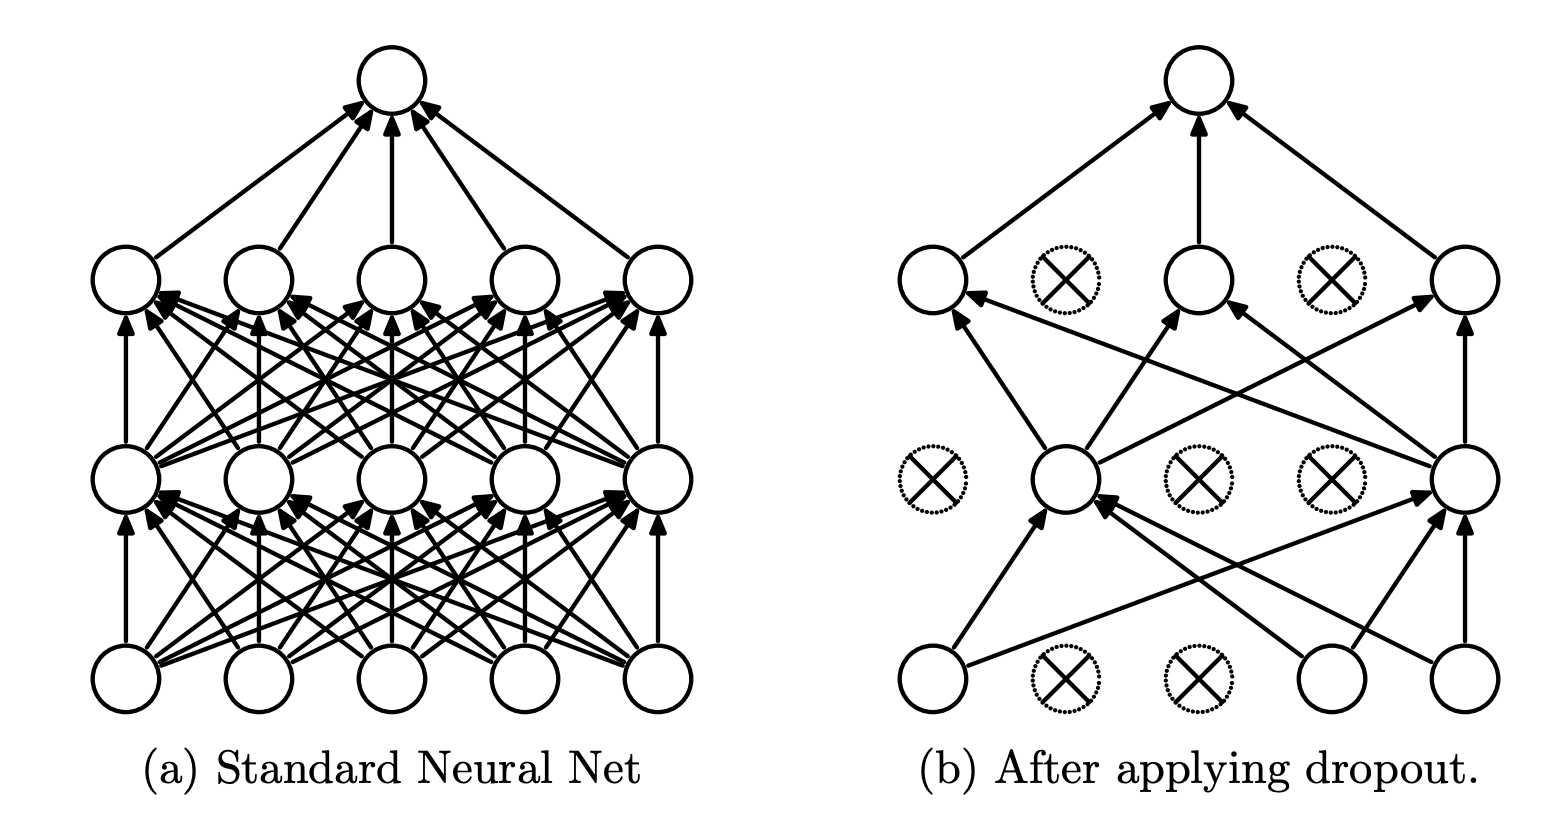
\includegraphics[width=0.8\linewidth]{bilder/dropout.png}
		\caption{Dropout}\label{fig:dropout}
	\end{center}
\end{figure}